\chapter{Quadcopter with artificial vision}\label{sec: Cuadricoptero}
In this chapter it is pretended to approach the design and development of a quad-copter which is able to follow an object, using for that a FPGA as a fundamental part and some other tools that will be exposed throughout this section. \newline

\section{Design}
In the following figure, a high abstraction level scheme is presented in which a first approach about the general system functionality is given. (\ref{fig:on_board}).

\begin{figure}[H]
	\center
	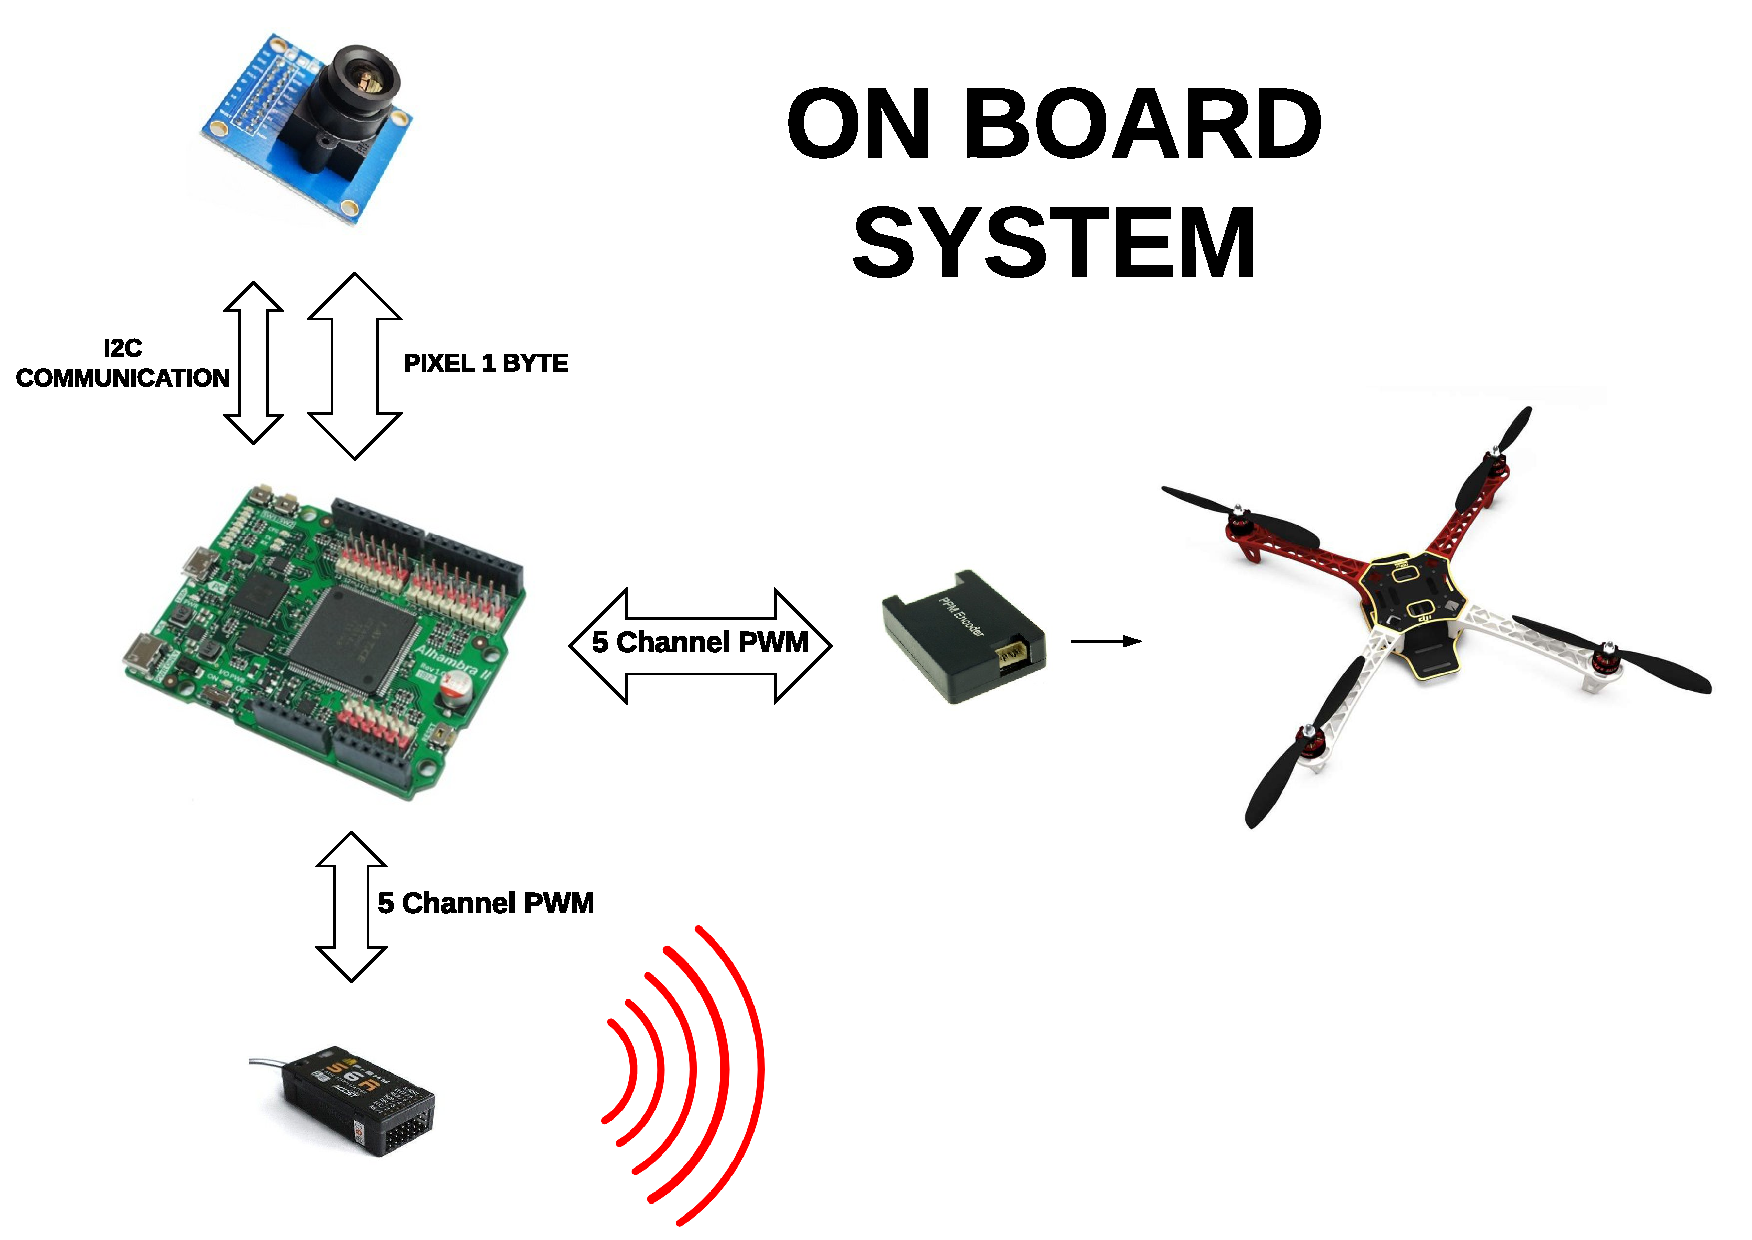
\includegraphics[trim = 0mm 0.5cm 0mm 0.5cm, clip,scale=0.4]{imagenes/Cuadricoptero_vision/on_board.pdf}
	\caption{Vision quad-copter high level design.}
	\label{fig:on_board}
\end{figure}

The design of this project has two parts, the part of stabilization control and the part of perception. As for the perception part, a low-cost camera will connect to the FPGA, which should implement the entire object recognition algorithm. Prior to this, and through the i2c protocol, the camera will be configured in such a way to make this recognition simpler. Subsequently and as an output of this recognition algorithm, the FPGA generates 4 PWM channels corresponding to the yaw, pitch, roll and altitude. It makes use of a PPM encoder, which transforms these 8 PWM signals into a PPM channel, input of the stabilization system of the quad-copter "Pixhawk".

\section{Perception Implementation}
Module OV7670\cite{OV7670} has a CMOS VGA image sensor OV7670, which allows to work at a maximum of 30 frames per second and a resolution of 640x480 pixels. It is a System on Chip (SoC) that is capable of processing images, such as: exposure control, gamma, white balance, color saturation, tone control. These parameters can be configured through the SCCB interface\cite{SCCB} (Serial Control Bus Camera).
Some of the most important features are presented below, and which could be obtained from its datasheet\cite{OV7670}.

\begin{itemize}
	\item 3.3 VDC Operation Voltage. 
	\item Sleep state current. $\mu$A
	\item 8 bits parallel data transmission. 
	\item SCCB Standard control Interface compatible with I2C. 
	\item optic objective 1/6” 
	\item Field of View (FOV): $25^{\circ}$C
	\item 640x480 VGA resolution
	\item 1.3V/(Lux-sex) sensibility 
	\item Signal to Noise Ratio: 46 dB. 
	\item High sensibility in low light environments. 
	\item Low voltage, according to portable applications
\end{itemize}
\newpage
An image from OV7670 module is pressent in Figure \ref{fig:OV7670}.

\begin{figure}[H]
	\center
	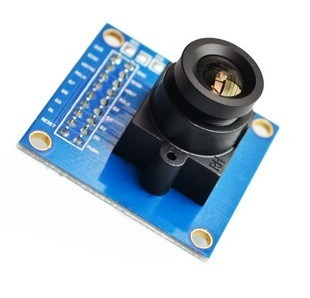
\includegraphics[scale=0.4, angle=0]{imagenes/Cuadricoptero_vision/OV7670}
	\caption{OV7670 camera.}
	\label{fig:OV7670}
\end{figure}

The camera configuration is done through an SCCB interface\cite{SCCB}, very similar to an I2C communication and whose registers can be found in the datasheet\cite{OV7670}. Therefore, it is necessary to choose a suitable configuration for this purpose:

\begin{itemize}
	\item A 640x480 window size is chosen because of the limited resources of the FPGA card used.
	\item The type of output data will be RGB, for the simplicity of use. We will therefore obtain two bytes for each pixel captured in the order represented in \ref{fig:pixel_OV7670}.
	
		\begin{figure}[H]
			\center
			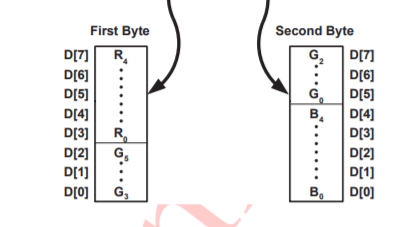
\includegraphics[trim = 0mm 0.5cm 0mm 0.5cm, clip,scale=0.6]{imagenes/Cuadricoptero_vision/pixel_OV7670}
			\caption{OV7670 Pixel Formation}
			\label{fig:pixel_OV7670}
		\end{figure}

	\item The velocity of adquisition in the outputs pixels has to be defined. This signal is in charge to notify when the next pixel can be captured. it is imposed that this signal is the half of the input clock. If the input clock frecuency is 12Mhz, the pixel signal generation will be 6MHz.
\end{itemize}

\subsubsection{I2C Protocol}

In order to achieve this configuration, an I2C communication is necessary with the OV7670 module that allows writing in certain records.

The appearance in IceStudio of this writing in I2C has the aspect of Figure \ref{fig:I2C_write}.
\begin{figure}[H]
	\center
	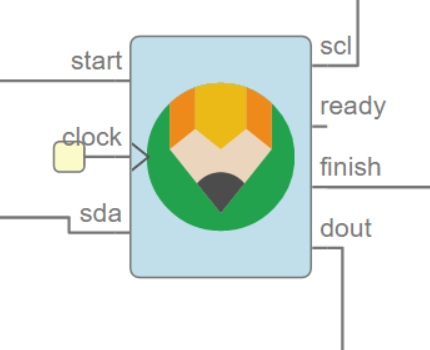
\includegraphics[scale=0.4, angle=0]{imagenes/Cuadricoptero_vision/I2C_write.PNG}
	\caption{I2C writing module in IceStudio aspect.}
	\label{fig:I2C_write}
\end{figure}

Since it has been an entirely module developed for this application, it is represented in the flow diagram in figure \ref{fig:i2c_write}.

\begin{figure}[H]
	\center
	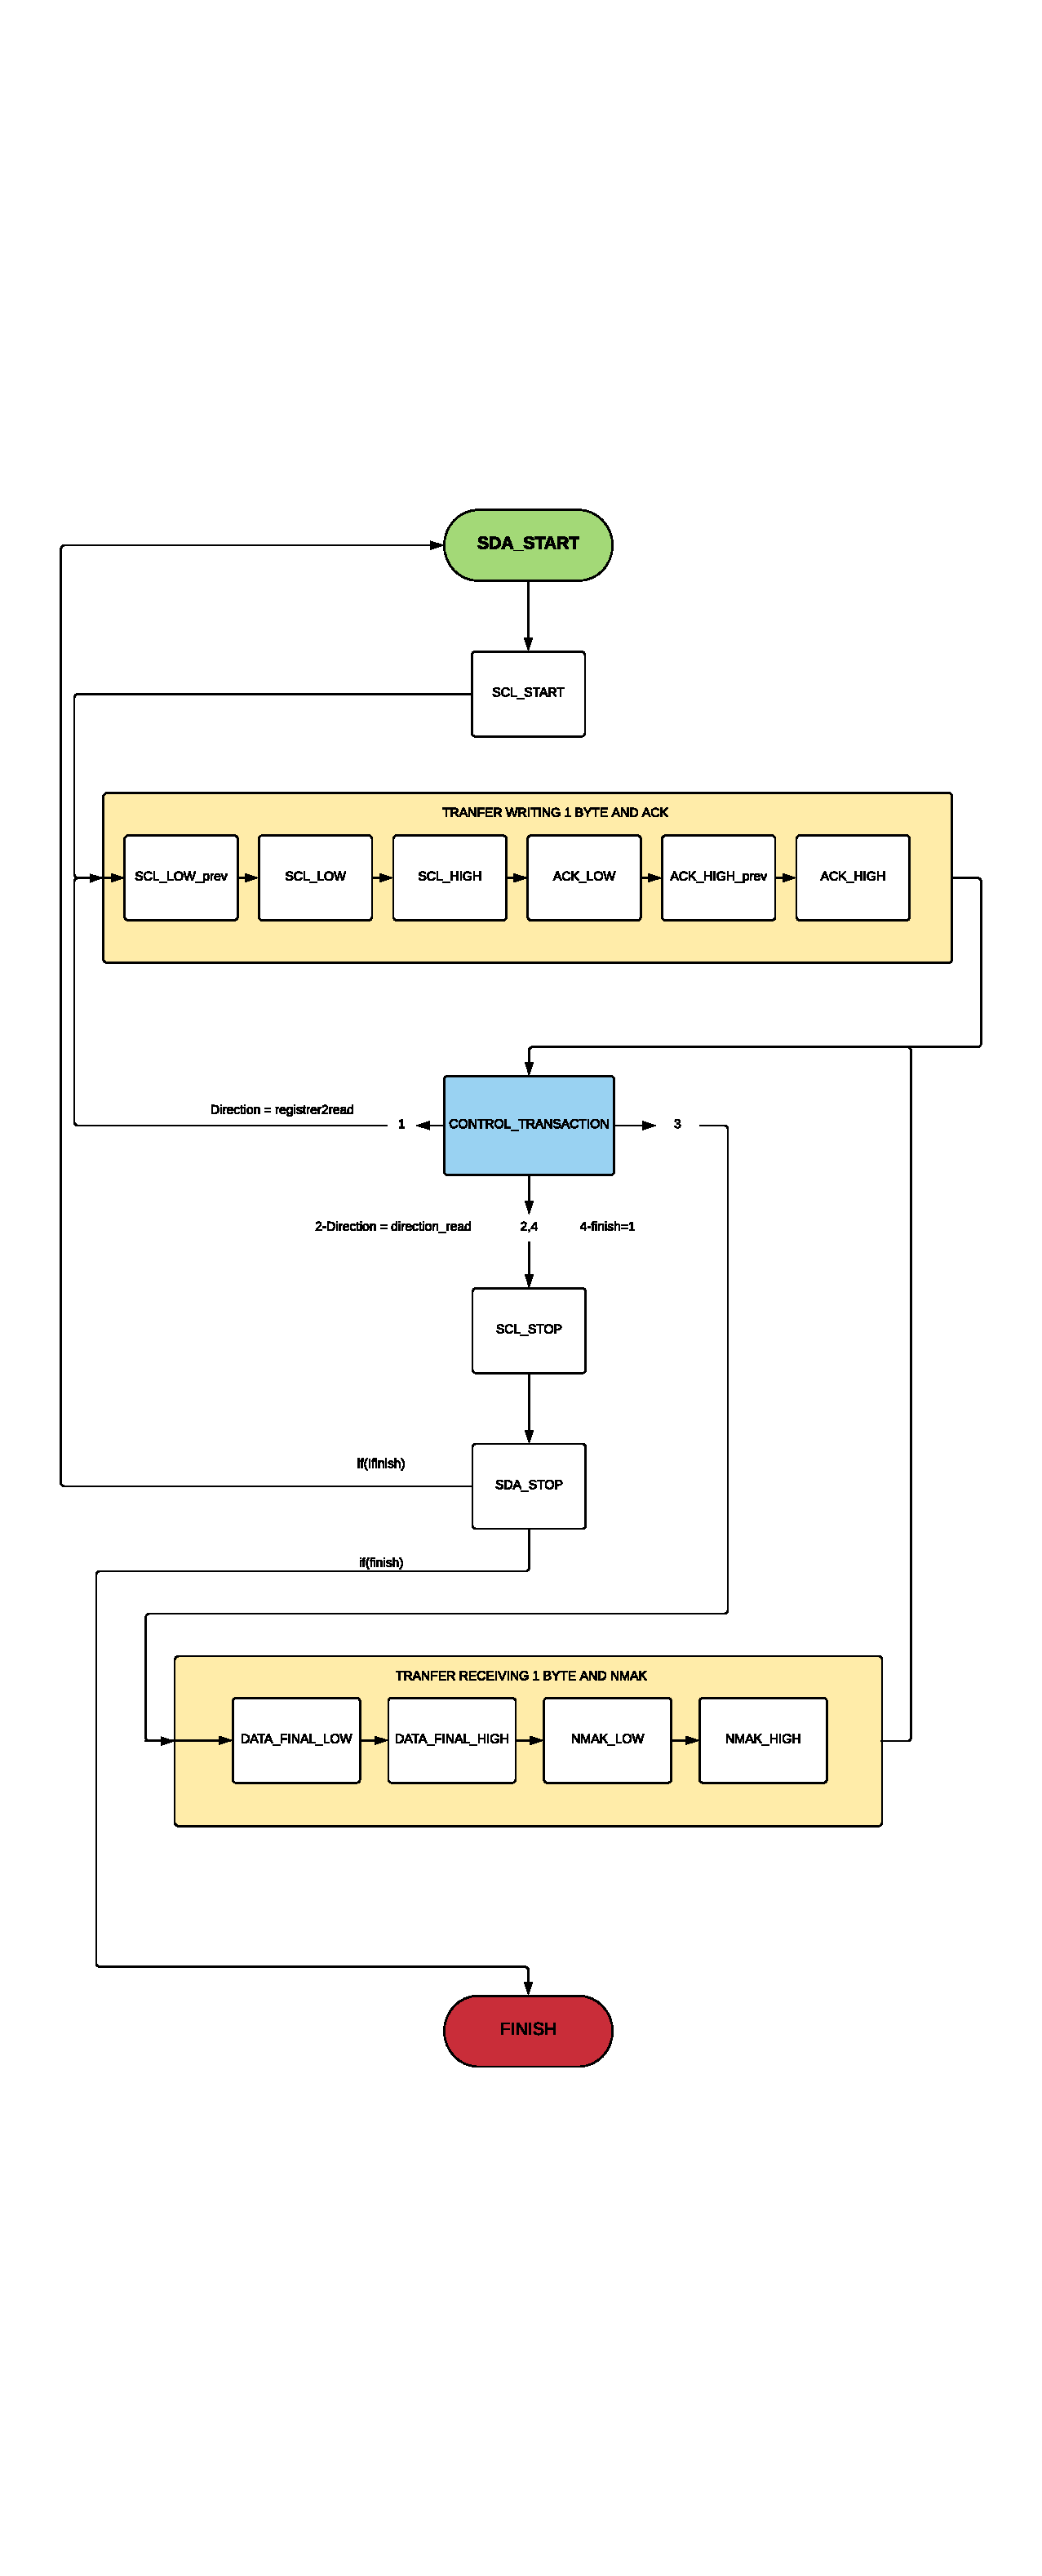
\includegraphics[trim = 0mm 6cm 0mm 6cm, clip,scale=0.5]{imagenes/Cuadricoptero_vision/I2C_WRITE.pdf}
	\caption{Flow diagram of I2C writing.}
	\label{fig:i2c_write}
\end{figure}

It is composed of a machine of 13 states in which each one has a fundamental function to achieve the desired result. You have to work at a very low level to avoid errors in the transmission and provide the system with the necessary tools for the detection of possible anomalies.

In an I2C communication it is important that both the master and the slave share the SCL and SDA buses, which will be always on high except when one of the two previous ones impose their path at a low voltage level, ground in this case. I2C bases it functionality in recognizing at every moment this voltage levels, which is why it is important to make sure that there is always the condition that if the bus is free, the voltage level is high. For that, both buses use to have a connection with a pull-up resistor that eases this feature and avoids at every moment possible clock glitches, bad ground reference, noise, etc. The connection schematics from the camera is below represented in figure \ref{fig:OV7670_schematic}.

\begin{figure}[H]
	\center
	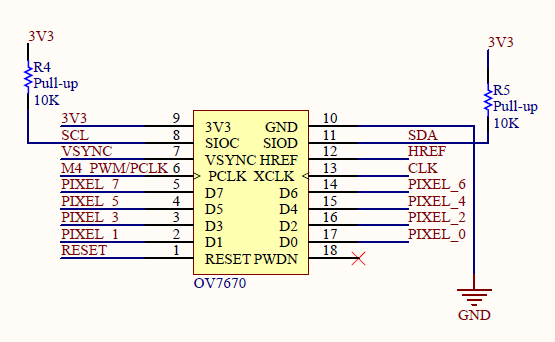
\includegraphics[scale=0.7, angle=0]{imagenes/Cuadricoptero_vision/OV7670_schematic}
	\caption{OV7670 camera schematics.}
	\label{fig:OV7670_schematic}
\end{figure}

One of the most important problem is this module’s development, which falls in temporal government of this buses by the slave and the master. For a better comprehension, it is described in example \ref{ejemplo:i2c}.

\begin{ejemplo}\label{ejemplo:i2c}
It is required at first instance that the master imposes the SDA bus at a high voltage level. Then, the master must be waiting for an answer coming from the slave, which is a non-controlled device and extern to our system. When the slave tries to write in the bus, it will find an imposed voltage level by the master which will not be able to be changed.
\end{ejemplo}

In order to correct the problem exposed in example \ref{ejemplo:i2c} the device waiting for a response much impose its high electric impedance state respect to the bus. This is why a tri-state bus is used which is represented in figure \ref{fig:buffer_triestado} and that allows this behavior in a controlled way.
\begin{figure}[H]
	\center
	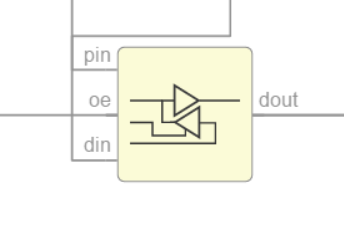
\includegraphics[scale=0.6, angle=0]{imagenes/Cuadricoptero_vision/triestado}
	\caption{Tri-state buffer for I2C bus.}
	\label{fig:buffer_triestado}
\end{figure}

A writing example in I2C in OV7670 module is represented in Figure \ref{fig:i2c_example}.

\begin{figure}[H]
	\center
	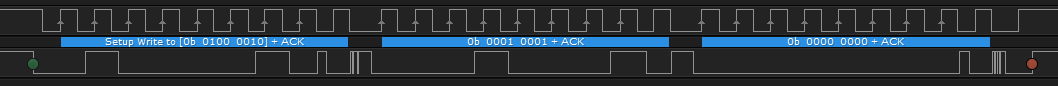
\includegraphics[scale=0.4, angle=0]{imagenes/Cuadricoptero_vision/i2c_example}
	\caption{I2C on OV7670 writing example.}
	\label{fig:i2c_example}
\end{figure}

\subsubsection{Pixels Storage}

One of the most important problems that must be solved when working with an OV7670 module and with the intention of objects recognizing in real time without delay, is the need for a FIFO memory that stores the pixels that are getting in, since to obtain a complete image of 640x480 it is necessary to store in memory 307200 pixels. In this case and considering that each cell is formed by two bytes, the total size of a frame will be the one shown in equation \ref{eq:pixeles}.

\begin{equation}\label{eq:pixeles}
	(640*480)*(16) = 4915200  \ \ \textup{bits por fotograma} 
\end{equation}

The device that controls the camera must be able to store that quantity of information so that later could be analyzed. \newline

In case of using a microcontroller, a FIFO memory could be incorporated to the system with the capacity to store that quantity of information. In this project it is used to the image analysis the FPGA IceZum Alhambra board and the shield exposed in \ref{sec:PCB}. The operating mode changes considerably compared to the previous one. \newline

After analyzing different alternatives, the most adequate and which a better performance could be reached, it is based in the no necessity to store a complete image, to understand this concept, it will be briefly explained in the section related to the position and volume of an object.
\newpage
\subsubsection{Volume and position recognize}\label{sec:volumen}

The recognition of the volume and positioning of the object will be calculated pixel by pixel instead of when obtained the complete image, thus the algorithm would be as follows:

\begin{itemize}
	\item At first instance, the color filter will be used, which will allow to recognize the color range of the pixel, in this case of the red ball. Therefore, a maximun and minimun will be defined for each red, green and blue component.
	\item Pixels will arrive sequentially, two bytes per pixels. The OV7670 module has as outputs pins D7, D6, D5, D4, D3, D2, D1, D0 corresponding to the bits of each component of the panel as shown in Figure \ref{fig:OV7670_schematic}.
	\item An internal counter will be in charge of keeping track of the number of total pixels that has passed through the filter. When the complete frame is finished, the object volume can be obtained, and with it, the distance to it, as shown in equation \ref{equation:filtro}.
	\begin{equation} \label{equation:filtro}
		Volume = Num_{\textup{filtered pixels}}/Num_{\textup{total pixels}}
	\end{equation}
	\item Considering the position within the frame where the pixels that have passed through the filter are, the position in columns and rows and from which you can obtain an estimate of the position of the object within the area of view as explained in equations \ref{equation:acumx3} and \ref{equation:acumy3}.
	
	\begin{equation}\label{equation:acumx}
		Acum_{X} = \sum\textup{columns of filtered pixels}
	\end{equation}
	
	\begin{equation}\label{equation:acumx2}
		X_{average} = \frac{Acum_{X}}{Num_{\textup{filtered pixels}}}
	\end{equation}

	\begin{equation}\label{equation:acumx3}
		Error_{X} = X_{average}- \frac{width}{2}
	\end{equation}
	
	\begin{equation}\label{equation:acumy}
		Acum_{Y} = \sum\textup{row filtered pixels}
 	\end{equation}
	
	\begin{equation}\label{equation:acumy2}
		Y_{average} = \frac{Acum_{Y}}{Num_{\textup{filtered pixels}}}
	\end{equation}
	
	\begin{equation}\label{equation:acumy3}
		Error_{Y} = Y_{average}- \frac{height}{2}
	\end{equation}
	
	\end{itemize}

To achieve the above behavior, it is therefore necessary to know at each exact moment what the value of the column and row in issue is.\newline
There are two independent modules developed; whose outputs provide these required positions.
	
	\begin{figure}[H]
		\center
		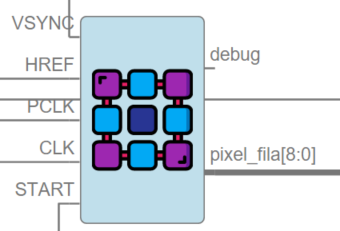
\includegraphics[scale=0.6, angle=0]{imagenes/Cuadricoptero_vision/filas_module}
		\caption{Row module in IceStudio.}
		\label{fig:filas_module}
	\end{figure}
	
	\begin{figure}[H]
		\center
		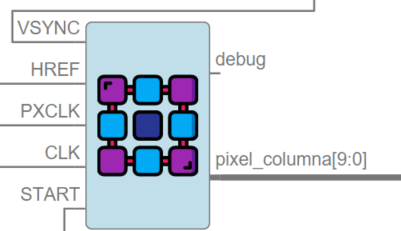
\includegraphics[scale=0.6, angle=0]{imagenes/Cuadricoptero_vision/columnas_module}
		\caption{Column module in IceStudio.}
		\label{fig:columnas_module}
	\end{figure}
	

	Due to the importance of these modules, the development of one of them is explained through its flow diagram exposed in figure \ref{fig:row_counter}.
	
	\begin{figure}[H]
		\center
		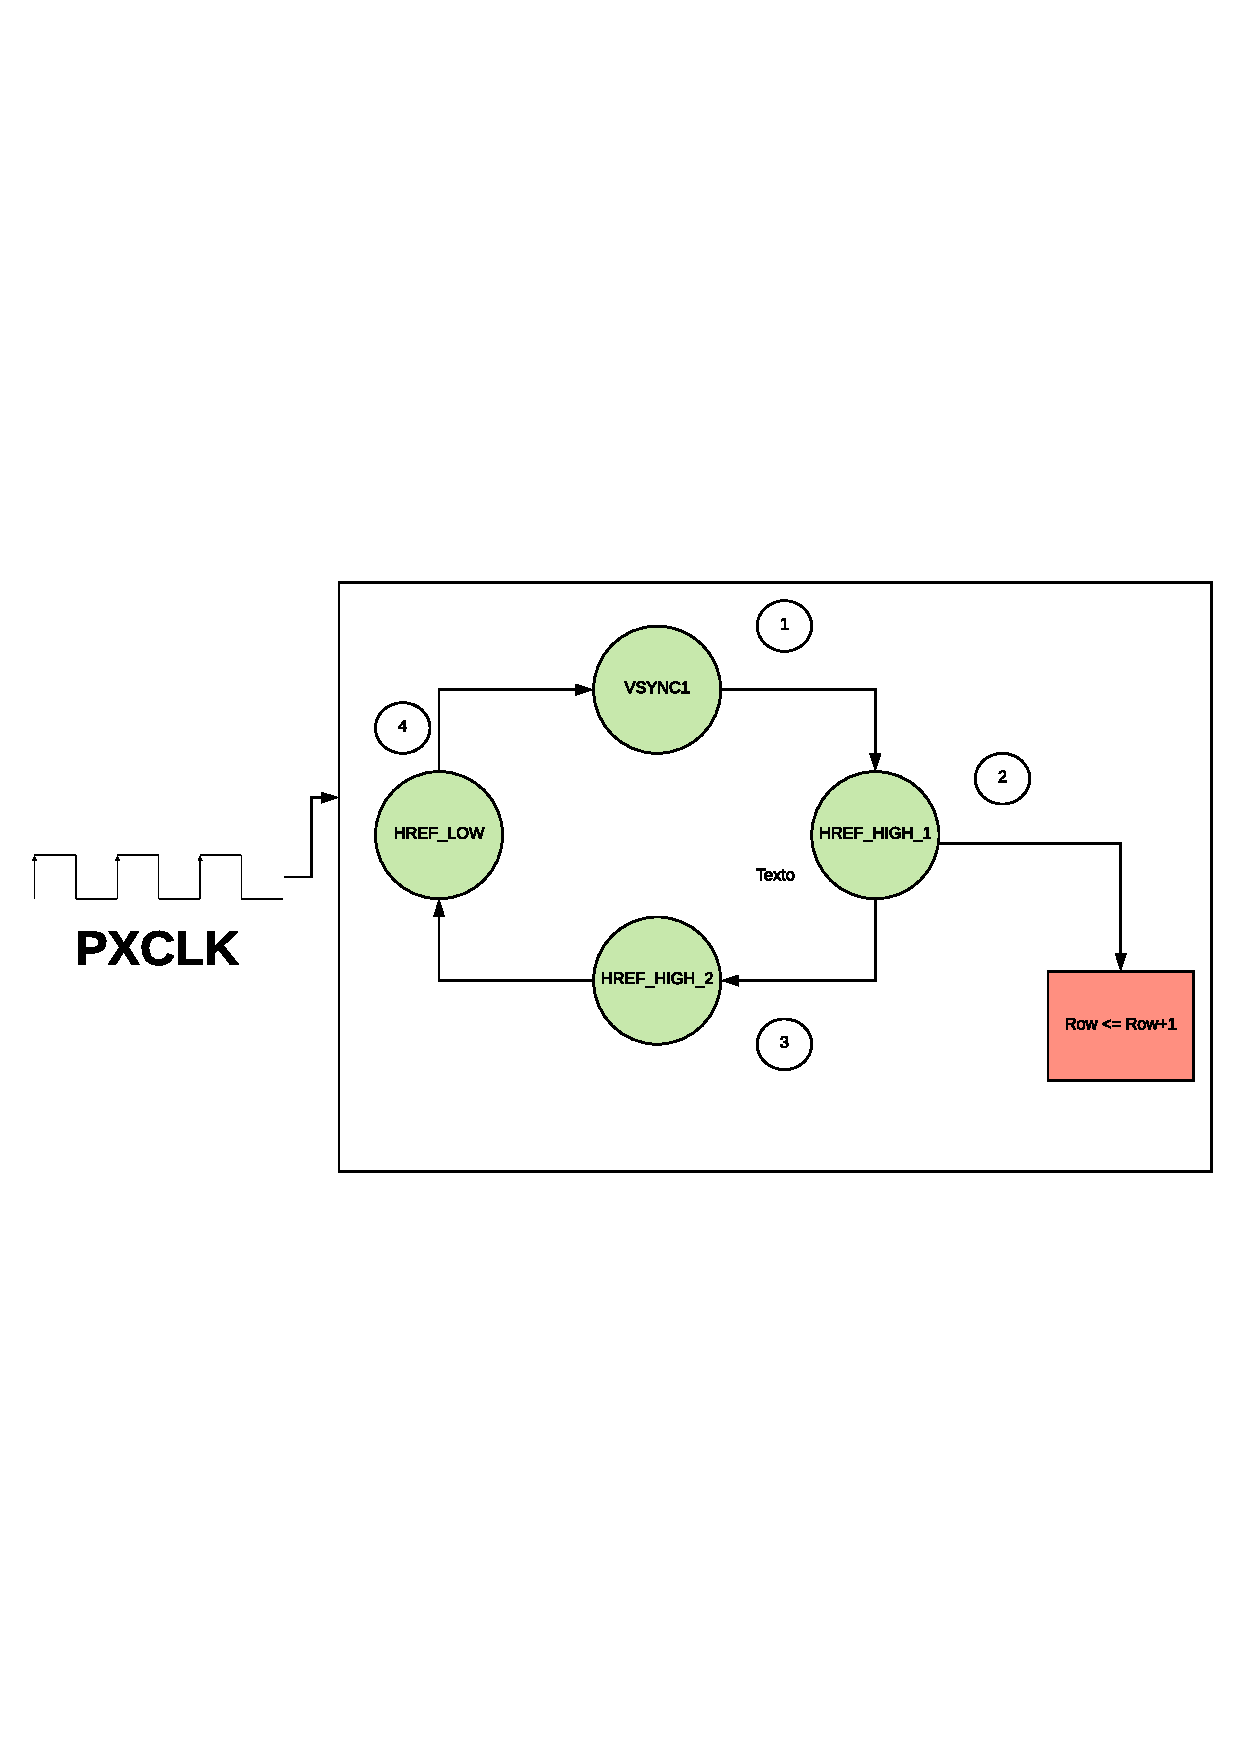
\includegraphics[trim = 0mm 8cm 0mm 8cm, clip,scale=0.5]{imagenes/Cuadricoptero_vision/row_counter.pdf}
		\caption{Flow diagram to the row counter.}
		\label{fig:row_counter}
	\end{figure}
	
	As is known, the OV7670 module provides a clock signal called PXCLK which will provide the synchronization of this module. On the other hand, it is important to know the synchrony signals with which every VGA signal count and which is represented in the figures \ref{fig:sincronismo}, \ref{fig:sincronismo1} y \ref{fig:sincronismo3}.
	
		\begin{figure}[H]
		\center
		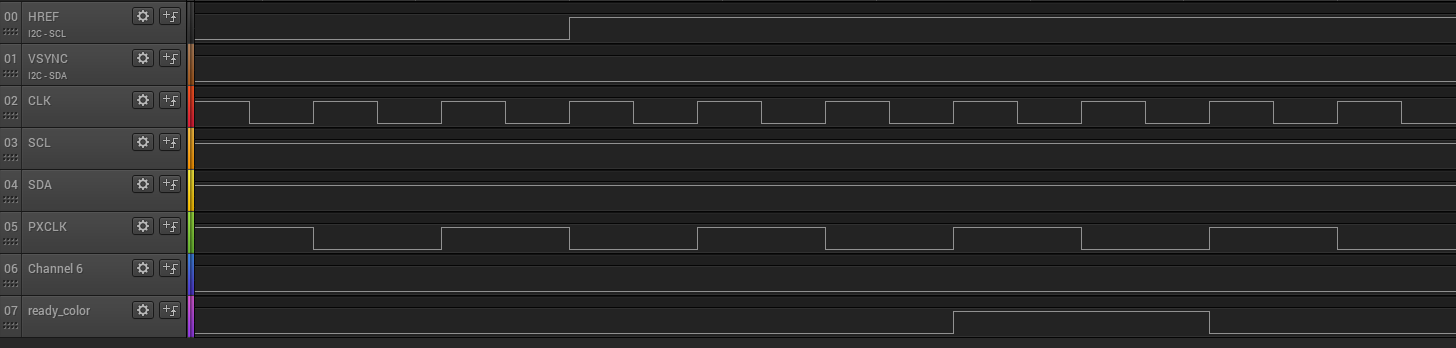
\includegraphics[scale=0.3, angle=0]{imagenes/Cuadricoptero_vision/sincronismo3}
		\caption{Synchronize signal OV7670.}
		\label{fig:sincronismo}
	\end{figure}
			\begin{figure}[H]
		\center
		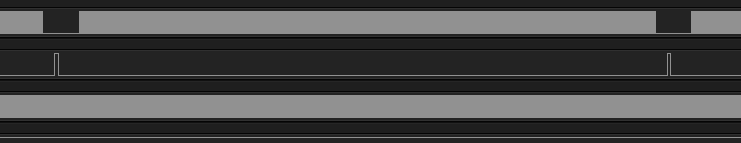
\includegraphics[scale=0.5, angle=0]{imagenes/Cuadricoptero_vision/sincronismo1}
		\caption{Synchronize signal OV7670.}
		\label{fig:sincronismo1}
	\end{figure}
			\begin{figure}[H]
		\center
		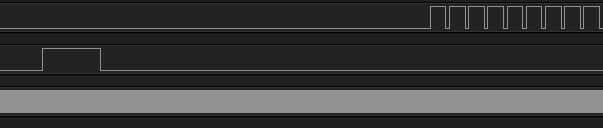
\includegraphics[scale=0.6, angle=0]{imagenes/Cuadricoptero_vision/sincronismo2}
		\caption{Synchronize signal OV7670.}
		\label{fig:sincronismo3}
	\end{figure}
	
There is a horizontal sync signal that will notify the change of the row in the frame and a vertical sync signal for the frame change.
	
	In the first place in the process of rows recognizing, it is necessary to detect when it begins and when it ends. A state machine has therefore been proposed in which each state assumes a change in the bus of the horizontal synchronization signal. 
	
	Once known the actual row and column, an auxiliar module is in charge to store the color components in different register. D7,D6,D5,D4,D3,D2,D1,D0 bits will be received wich correspond with red component and the three most significative bits of green component as it is indicated in \ref{equation:byte1}.
	
	\begin{equation} \label{equation:byte1}
		RED = (D7,D6,D5,D4,D3)
	\end{equation}
	
	\begin{equation*}
		GREEN_{prev} = (D2,D1,D0)
	\end{equation*}
	
	In second place, the second byte will be received with the other green part and the hole blue component (\ref{equation:byte2}).
	
	\begin{equation} \label{equation:byte2}
	GREEN = (GREEN_{prev},D7,D6,D5)
	\end{equation}
	
	\begin{equation*}
	BLUE = (D4,D3,D2,D1,D0)
	\end{equation*}
	
	The behaviour showed in equations \ref{equation:byte1} and \ref{equation:byte2} can be developed with a state machine as it is represented in \ref{fig:assign_pixel}. PXCLK is used as sensibility list.
	
		\begin{figure}[H]
		\center
		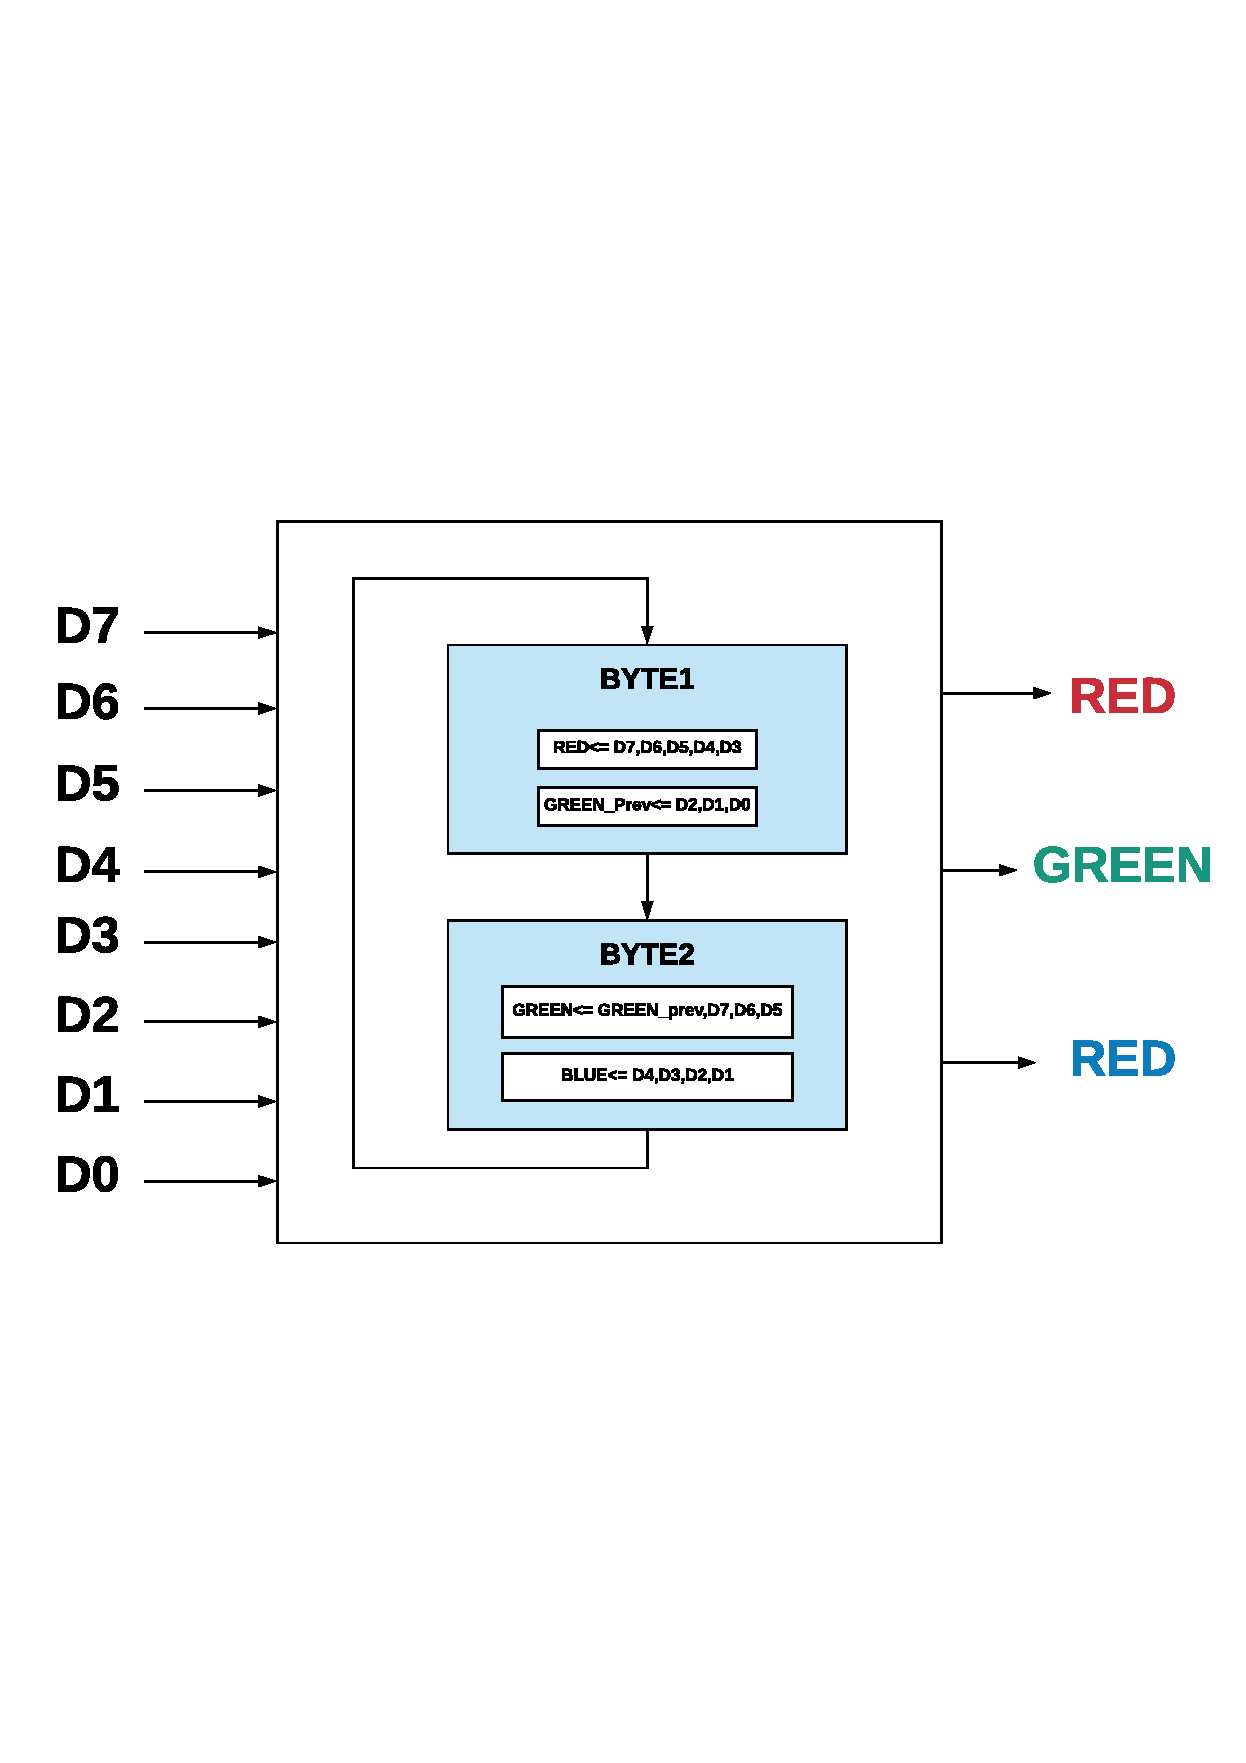
\includegraphics[trim = 0mm 6cm 0mm 6cm, clip,scale=0.5]{imagenes/Cuadricoptero_vision/assign_pixel.pdf}
		\caption{Bits assigments.}
		\label{fig:assign_pixel}
	\end{figure}

	The final appearance of this module is represented in figure \ref{fig:assign_bits}.
	
		\begin{figure}[H]
		\center
		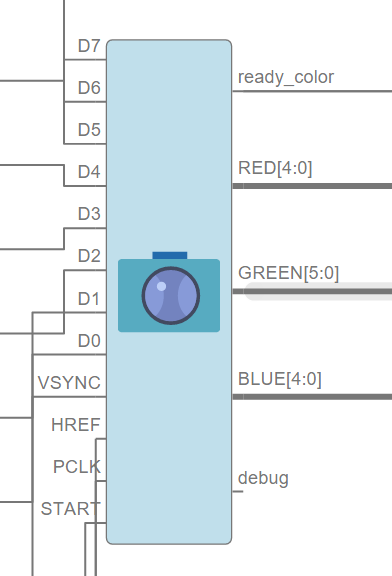
\includegraphics[scale=0.6, angle=0]{imagenes/Cuadricoptero_vision/assign_bits}
		\caption{Bits assigments in IceStudio.}
		\label{fig:assign_bits}
	\end{figure}
	
 
 	 If it is observed in figure \ref{fig:assign_bits} in the output of this module the three color components will be obtained and a signal will be in charge to notify when the three color components are ready.\newline
	
	The next module has enough iformation to implement the whole showed algorithm in \ref{sec:volumen}.

\section{Control Design}

Respect to the control implementation on quadcopter board, it is presented only the theorical basis in order to improves it in following works. 

To understand this behaviour, the figure  \ref{fig:control_implemtation} is represented.

\begin{figure}[H]
	\center
	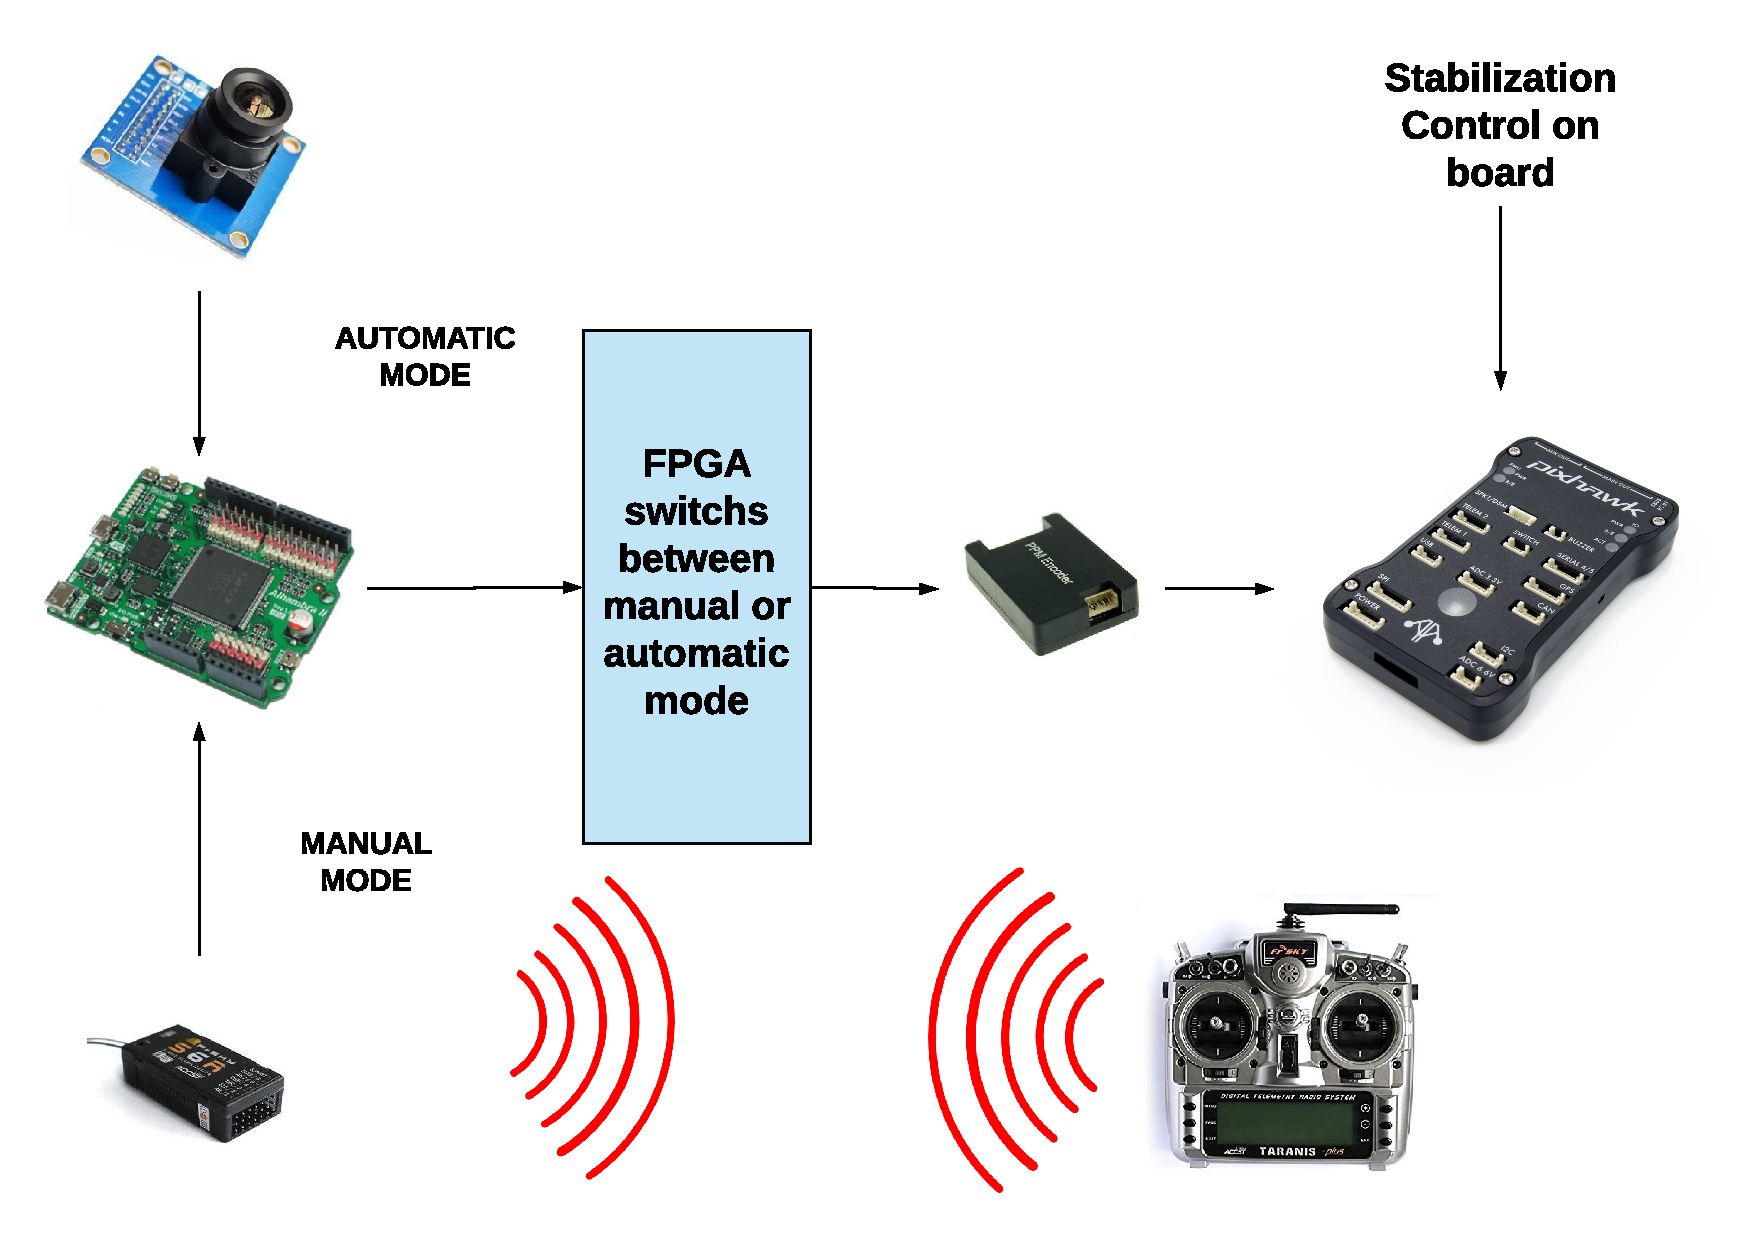
\includegraphics[trim = 0mm 0cm 0mm 0cm, clip,scale=0.4]{imagenes/Cuadricoptero_vision/control_implementation.pdf}
	\caption{Diagram of control Implementation.}
	\label{fig:control_implemtation}
\end{figure}


The stabilization control will take part of the inter processes from PixHawk board. This has a PPM signal connected corresponding to the reception of the signal coming from a frequency transmitter, which sends the PWM signal from the Yaw, Pitch and Roll. \newline

The objetive is to modify this signal wich provoke the quadcopter movement in relation with the output recognition object protocol. The FPGA will be in the middle between signal receptor (FrSky) and PixHawk in order to allow the both behaviour. 

Both behaviour can be:

\begin{itemize}
	\item Automatic mode: The quad-copter will move in relation to the object, having as a principal objective it is positioned at the center of the vision area. To maximize this tracing a PID control an be used which is developed in this project. Quadcopter will move in relation to the position of the object being detected.
	\item Manual mode: Quadcopter will move in relation to the signal received from the radio transmitter.
\end{itemize}
